\documentclass[crop=false]{standalone}
%\documentclass{standalone}
\usepackage{tikz} % To generate the plot from csv
\usepackage{pgfplots}
\usepackage{graphicx}
\usepackage{booktabs}
\usepackage{subfig}
\usepackage{float}
\usepackage[section]{placeins} % getting figures below sections
\usepackage{blindtext}
\usepackage{siunitx}
\usepgfplotslibrary{units} % Allows to enter the units nicely
\usetikzlibrary{external} %https://tex.stackexchange.com/questions/1460/script-to-automate-externalizing-tikz-graphics
\tikzexternalize[prefix=savedfigures/]

\pgfplotsset{compat=newest} % Allows to place the legend below plot
\usepackage{pgfplotstable}
\usepgfplotslibrary{statistics}

% #################### Function definition for box plots read table ##################\
\makeatletter
\pgfplotsset{
	boxplot prepared from table/.code={
		\def\tikz@plot@handler{\pgfplotsplothandlerboxplotprepared}%
		\pgfplotsset{
			/pgfplots/boxplot prepared from table/.cd,
			#1,
		}
	},
	/pgfplots/boxplot prepared from table/.cd,
	table/.code={\pgfplotstablecopy{#1}\to\boxplot@datatable},
	row/.initial=0,
	make style readable from table/.style={
		#1/.code={
			\pgfplotstablegetelem{\pgfkeysvalueof{/pgfplots/boxplot prepared from table/row}}{##1}\of\boxplot@datatable
			\pgfplotsset{boxplot/#1/.expand once={\pgfplotsretval}}
		}
	},
	make style readable from table=lower whisker,
	make style readable from table=upper whisker,
	make style readable from table=lower quartile,
	make style readable from table=upper quartile,
	make style readable from table=median,
	make style readable from table=average,
	make style readable from table=lower notch,
	make style readable from table=upper notch
}
\makeatother
\begin{document}

\section{24 2 Mumford0 SA Mutations more 20210817 144535}

% ######################## UTRP SA Mutation operators applied ######################## 
\begin{figure} 
\centering 
\tikzsetnextfilename{UTRP_DBMOSA_BP_mutation_funcs_more} 
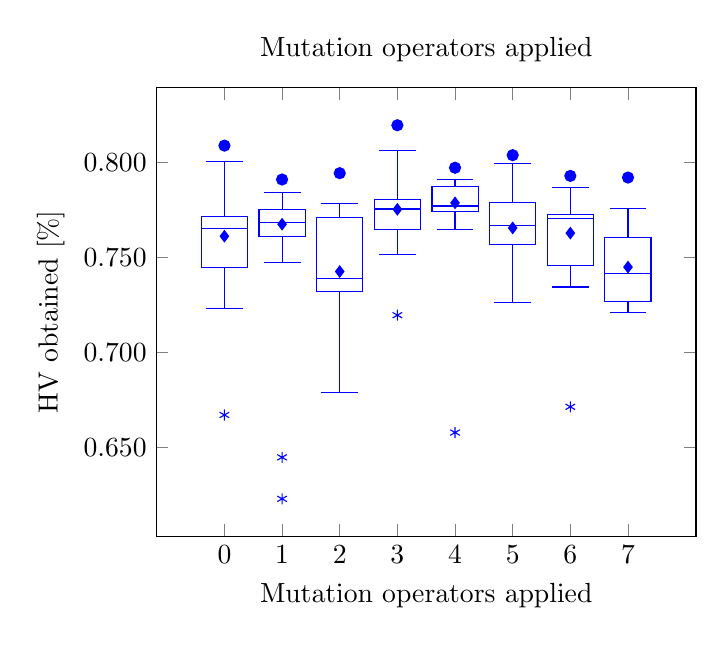
\begin{tikzpicture} 
\begin{axis}[ 
title={Mutation operators applied}, 
boxplot/draw direction=y, 
xtick={1,2,3,4,5,6,7,8}, 
xticklabels={0,1,2,3,4,5,6,7}, 
x tick label style={rotate=0, align=center}, 
xlabel={Mutation operators applied}, 
y tick label style={/pgf/number format/.cd,fixed,precision=3, zerofill}, 
ylabel={HV obtained [\%]}, 
] 

% ############## Mutations_more=0 ################## 
\addplot[boxplot, mark=asterisk, 
boxplot prepared={ 
lower whisker=0.72313, 
upper whisker=0.80046, 
lower quartile=0.74462, 
upper quartile=0.77158, 
median=0.76494, 
average=0.76106}, 
color = blue, solid, area legend] 
coordinates {
(1,0.66703)}; 
\addplot[only marks,mark=*,color = blue]coordinates{(1,0.8087)}; 

% ############## Mutations_more=1 ################## 
\addplot[boxplot, mark=asterisk, 
boxplot prepared={ 
lower whisker=0.74709, 
upper whisker=0.78409, 
lower quartile=0.76073, 
upper quartile=0.77511, 
median=0.76848, 
average=0.76736}, 
color = blue, solid, area legend] 
coordinates {
(2,0.64474)
(2,0.62292)}; 
\addplot[only marks,mark=*,color = blue]coordinates{(2,0.79088)}; 

% ############## Mutations_more=2 ################## 
\addplot[boxplot, mark=asterisk, 
boxplot prepared={ 
lower whisker=0.67887, 
upper whisker=0.77832, 
lower quartile=0.73178, 
upper quartile=0.77099, 
median=0.73888, 
average=0.74246}, 
color = blue, solid, area legend] 
coordinates {}; 
\addplot[only marks,mark=*,color = blue]coordinates{(3,0.7942)}; 

% ############## Mutations_more=3 ################## 
\addplot[boxplot, mark=asterisk, 
boxplot prepared={ 
lower whisker=0.75152, 
upper whisker=0.80623, 
lower quartile=0.76475, 
upper quartile=0.78014, 
median=0.77536, 
average=0.77517}, 
color = blue, solid, area legend] 
coordinates {
(4,0.71951)}; 
\addplot[only marks,mark=*,color = blue]coordinates{(4,0.81942)}; 

% ############## Mutations_more=4 ################## 
\addplot[boxplot, mark=asterisk, 
boxplot prepared={ 
lower whisker=0.7644, 
upper whisker=0.79103, 
lower quartile=0.77414, 
upper quartile=0.78715, 
median=0.77692, 
average=0.77857}, 
color = blue, solid, area legend] 
coordinates {
(5,0.65779)}; 
\addplot[only marks,mark=*,color = blue]coordinates{(5,0.79706)}; 

% ############## Mutations_more=5 ################## 
\addplot[boxplot, mark=asterisk, 
boxplot prepared={ 
lower whisker=0.72622, 
upper whisker=0.79923, 
lower quartile=0.75668, 
upper quartile=0.77855, 
median=0.76647, 
average=0.76541}, 
color = blue, solid, area legend] 
coordinates {}; 
\addplot[only marks,mark=*,color = blue]coordinates{(6,0.80368)}; 

% ############## Mutations_more=6 ################## 
\addplot[boxplot, mark=asterisk, 
boxplot prepared={ 
lower whisker=0.73436, 
upper whisker=0.78687, 
lower quartile=0.74548, 
upper quartile=0.77269, 
median=0.77023, 
average=0.76268}, 
color = blue, solid, area legend] 
coordinates {
(7,0.67132)}; 
\addplot[only marks,mark=*,color = blue]coordinates{(7,0.79278)}; 

% ############## Mutations_more=7 ################## 
\addplot[boxplot, mark=asterisk, 
boxplot prepared={ 
lower whisker=0.72097, 
upper whisker=0.77555, 
lower quartile=0.72654, 
upper quartile=0.76051, 
median=0.74158, 
average=0.7448}, 
color = blue, solid, area legend] 
coordinates {}; 
\addplot[only marks,mark=*,color = blue]coordinates{(8,0.79191)}; 

\end{axis}
\end{tikzpicture}
\end{figure} 
\begin{table}
\centering
\caption{Legend for the boxplot.}
\begin{tabular}{ll}
\toprule
 Index &                                               Name \\
\midrule
     0 & [Add\_vertex, Delete\_vertex, Insert\_inside\_verte... \\
     1 & [MSC\_add\_terminal, MSC\_del\_terminal, Insert\_ins... \\
     2 & [Trim\_one\_terminal\_cb, Grow\_one\_terminal\_cb, In... \\
     3 & [Intertwine\_two, Add\_vertex, Delete\_vertex, Inv... \\
     4 & [Intertwine\_two, MSC\_add\_terminal, MSC\_del\_term... \\
     5 & [Intertwine\_two, Trim\_one\_terminal\_cb, Grow\_one... \\
     6 & [Intertwine\_two, Add\_vertex, Delete\_vertex, Inv... \\
     7 & [Intertwine\_two, MSC\_add\_terminal, MSC\_del\_term... \\
\bottomrule
\end{tabular}
\end{table}

\end{document}
